
\chapter{Osnovni pojmovi} % Main chapter title


%------------------------------------------------------------------------------

Svi živi organizmi sastoje se od jedne ili više ćelija, a svaka ćelija od
molekula. Veliki\footnote{ Obično se molekulska masa od $1000 Da$ (Daltona) uzima kao 
granica između malih molekula i makromolekula.}
molekuli (makromolekuli) organskog porekla obično\footnote{
  Lipidi recimo nisu polimeri, ali su principijalno slični
} su sačinjeni od
ponavljajućih strukturnih jedinica \keyword{monomera} \textit{(mono- = jedan,
mer- = deo)} međusobno povezanih \keyword{kovalentnim} vezama.  Takav molekul
zovemo \keyword{polimer} \textit{(poli- =mnogo, -mer= deo)}. 
% Polimer može da bude \textit{homo-polimer}, sačinjen od jednog tipa monomera
% ili suprotno \textit{hetero-polimer}, sačinjen od nekoliko raznih tipova
% monomera.
Skup monomera možemo da smatramo azbukom koja gradi jezik polimera.  Mali broj
monomera je dovoljan za strukturnu kompleksnost bilo koje ćelije.  Tri 
najznačajnija tipa bioloških polimera i njihovi monomeri prikazani su u Tabli
\ref{tab:polimeri}.

\begin{table}[htpb]
  \centering
  \caption{Najznačajniji biološki polimeri}
  \label{tab:polimeri}
  \begin{tabular}{ll}
    \keyword{Polimer}            & \keyword{Monomer} \\
    Ugljeni hidrati              & Monosaharid (šećeri) \\
    Nukleinska kiselina (DNK)    & Nukleotid \\
    Protein                      & Aminokiselina \\
    \hline
  \end{tabular}
\end{table}


\section{Centralna dogma molekularne biologije}

Centralna dogma molekularne biologije prikazana Slikom \ref{fig:dogma}
objašnjava protok informacija kroz generacije i ćeliju.

\begin{figure}[th]
\centering
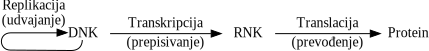
\includegraphics[]{uvod/centralna_dogma}
\caption { Centralna dogma molekularne biologije }
\label{fig:dogma}
\end{figure}


Dezoksiribonukleinska kiselina, kraće \keyword{DNK} se procesom replikacije
(tokom deobe ćelije) udvaja u dve kopije. Tokom života ćelije regioni DNK
molekula tzv. \keyword{geni} bivaju transkribovani (prepisani) u oblik
ribonukleinske kiseline, kraće \keyword{RNK}.  Glasnička RNK, kraće mRNK
dobijena transkripcijom tzv. kodirajućeg gena sadrži kodirane informacije
potrebne za sintezu proteina i biva transportovana do molekulskih mašina
ribozoma. Ribozom translira (prevodi) mRNK u protein. Pomenuti kod prikazan
Slikom \ref{fig:kod} zove se \keyword{genetički kod} i opisuje mapiranje nukleinskih
trigrama tzv.  \keyword{kodona} u aminokiseline ili stop oznaku.

\begin{figure}[]
\centering
\hspace*{-2.3cm} 
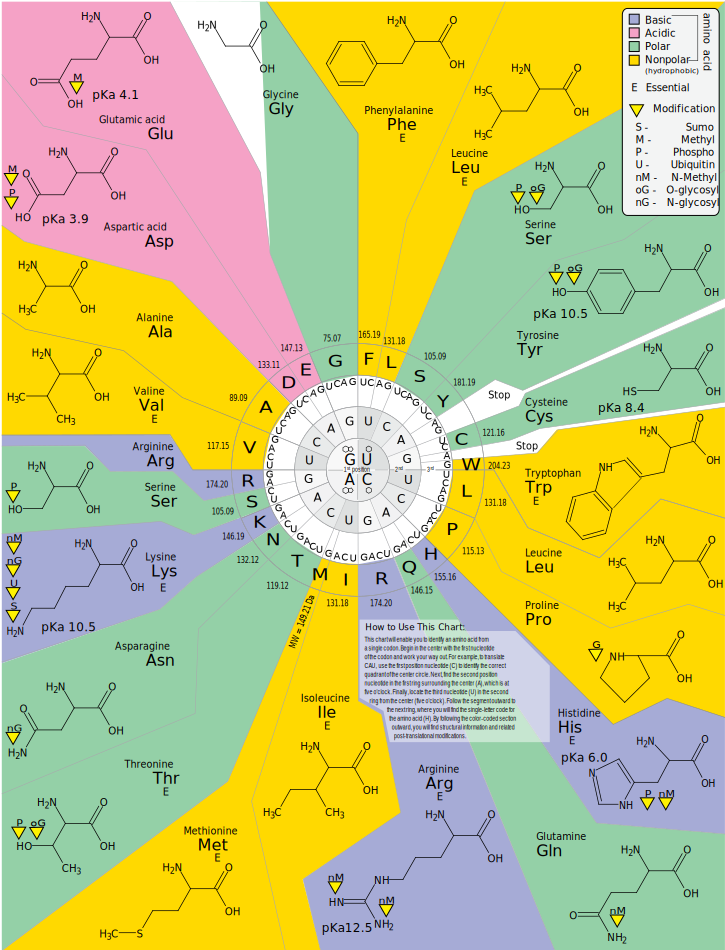
\includegraphics[scale=0.94]{uvod/geneticcode22}
\caption { Genetički kod, aminokiseline, osobine AK i lokacije PTM\\
  \footnotesize
Originalna Slika pripada vikimedija javnom domenu (autor Bromomir)}
\label{fig:kod}
\end{figure}

\clearpage

Genetički kod je univerzalan\footnote{Postoje izuzeci kod malog broja
organizama koji neke kodone prevode drugačije ili proširuju mapiranje
nestandardnim aminokiselinama} za sva živa bića.  Kompletan DNK kod nekog
organizma predstavlja njegov \keyword{genom}.  Gen je region DNK sekvence koja
biva transkribovana u RNK.  Neki geni su tzv. nekodirajući geni i transkribuju
se u funkcionlane RNK molekule.  Svi produkti transkripcije gean (RNK) čine
\keyword{transkriptom}, dok svi sintetisani proteini čine \keyword{proteom}.
Tri velike oblasti bioinformatike koje prikupljaju i analiziraju ove podatke
su: \keyword{genomika}, \keyword{transkriptomika} i \keyword{proteomika}.


\label{sec:}
\section{Proteini}

Proteini (belančevine) su najčešći biološki makromolekuli koji čine i do $80\%$
suve mase organizma.  Strukturno, protein je linearan polimer sačinjen od lanca
\keyword{aminokiselina}(monomeri) skraćeno AK. Iako u prirodi postoje stotine
različitih aminokiselina, kod svih živih organizama javlja se samo 20 tzv.
''standardnih'' aminokiselina\footnote{Izuzetak, Selenocistein i Pirolizin su tzv 21. i
22. aminokiselina i javljaju se samo kod nekih mikroorganizama}.

Standardne aminokiseline imaju šablon strukturu predstavljenu Slikom \ref{fig:AK} a).
Centralni alfa ugljenikov atom ($C_{\alpha}$) povezan je sa amino grupom ($-NH_2$), 
karboksilnom grupom ($-COOH$), atomom vodonika i tzv. R grupom. Dvadeset aminokiselina
razlikujemo po R grupi još poznatoj kao bočni niz ili bočni ostatk \en{residue}.
Prema hemijskim osobinama bočnog niza aminokiseline se mogu klasifikovati na
nekoliko načina prikazanih na Slikama \ref{fig:AK_vene} i \ref{fig:kod} od
čega izdvajamo sledeću podelu:
\begin{itemize}
  \item Nepolarne AK -
    zbog manjka asimetrije u naelektrisanju R grupe ovi molekuli nisu
    rastvorljivi u vodi (koja je polaran molekul). Hidrofobni su (ne vole
    vodu).  Obično ove aminokiseline se nalaze u unutrašnjosti savijenog proteina gde
    je kontakt sa vodom mimimalan.
    
  \item Nenaelektrisane polarne AK -
    su više rastvorljive u vodi (vole vodu).  Uglavnom se nalaze na spoljim
    delovima proteina, često na hemijski aktivnim delovima.

  \item Naelektrisane polarne AK -
    su jako hidrofilne. Dodatno se dele na pozitivno i negativno naelektrisane.

  \item Aromatične AK - su među najvećim i najtežim jer u bočnom nizu sadrže
    aromatični ugljenikov prsten.
\end{itemize}

Reakcijom kondenzacije prikazane na Slici \ref{fig:AK} b) dve aminokiseline
grade kovalentnu tzv. peptidnu vezu. Rezultat reakcije je peptid (dipeptid) dok
duže lance aminokiselina (preko 10 AK) prikazane Slikom \ref{fig:AK} c)
nazivamo polipeptidima ili proteinima. Peptid ima smer pri čemu razlikujemo
početak, N-terminus i kraj, C-terminus.
\clearpage

\begin{figure}[th]
\centering
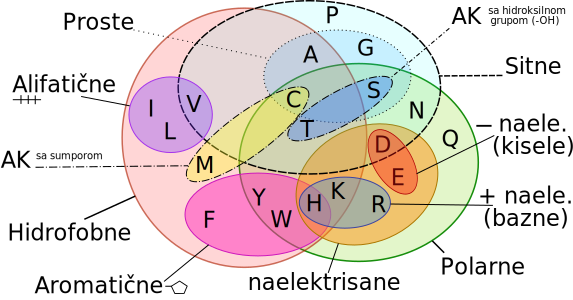
\includegraphics[scale=0.9]{uvod/AK_vene.pdf}
\caption {Veneov dijagram osobina bočnih nizova aminokiselina}
\label{fig:AK_vene}
\end{figure}

\begin{figure}[th]
\centering
% \hspace*{-2.0cm} 
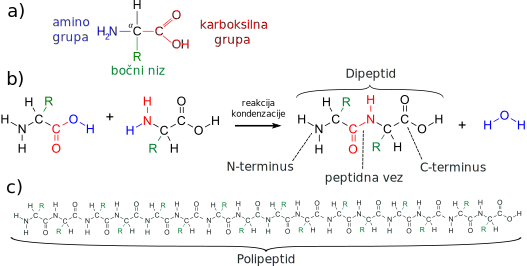
\includegraphics[scale=0.8]{uvod/aminokiselina.pdf}
\caption {a) Šematski priakz aminokiseline
b) spajanje aminokiselina reakcijom kondenzacije
c) Šematski prikaz polipeptida
}
\label{fig:AK}
\end{figure}


\subsection{Struktura proteina}

Proteini su formirani iz jednog ili više polipeptidnih lanaca. Njihova struktura
opisuje se kroz četiri nivoa rastuće složenosti.

\keyword{Primarna struktura} opisana je redosledom peptidnih veza polipetidnog
lanca, odnosno redosledom AK.  Primarna struktura predstvalja \keyword{sekvencu
proteina} i kompaktno je predstavljamo azbukom od minimum 20 slova.

\keyword{Sekundardna struktura} najčešće nastaje formiranjem vodoničnih veza
između atoma kiseonika i azota koje indukuju dva oblika prikazana Slikom \ref{fig:sekundarna}:
\begin{itemize}
  \item \keyword{alfa spirala} - je spiralna struktura u kojoj R grupe štrče spolja
  \item \keyword{beta ploča}  - predstavlja spoj dva ili više (anti)paralelnih delova pp. lanca
\end{itemize}
Pored gore navedenih, strukture: disulfidni most\footnote{Neki autori
disulfidni most smatraju za elemenat primarne strukture}, zink prsti i ukosnica
takođe se smatraju za elemente sekundarne strukture.

\begin{figure}[th]
\centering
\hspace*{-2.0cm} 
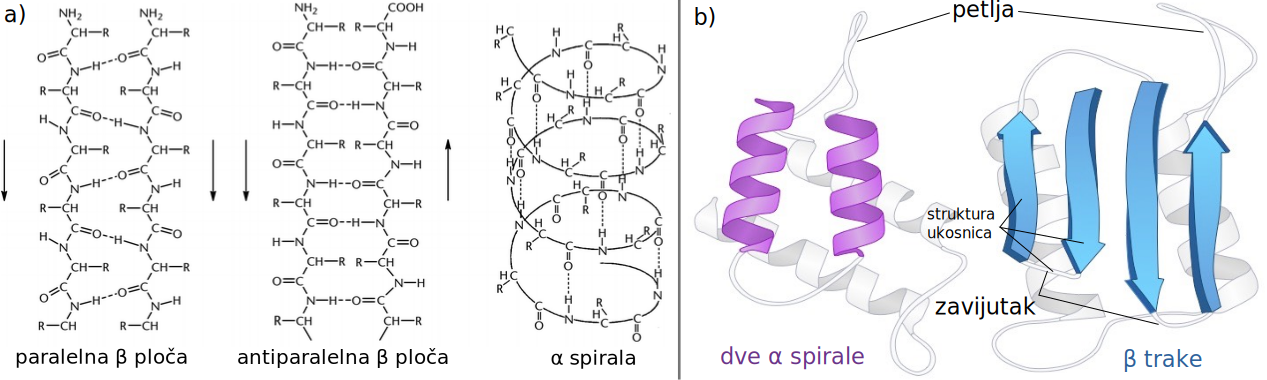
\includegraphics[scale=0.53]{uvod/sekundarna.pdf}
\caption {
  Alfa spirala i beta ploče.\\ \footnotesize Levi deo slike preuzet je iz rada
  \textit{Proteins: fundamental chemical properties. Cozzone, A. J.
  Encyclopedia of Life Sciences (Nature Publishing Group, London, 2001)}.
  Desni deo slike preuzet je sa veb strane bioninja.com
}
\label{fig:sekundarna}
\end{figure}


\keyword{Tercijarna struktura} je prostorni oblik koji polipeptid zauzima indukvan 
interakcijama bočnih nizova aminokiselina.  Pod poznavanjem tercijarne
strukture misli se na poznavanje prostornih kordinata svih atoma polipeptida.
Najveći uticaj na oblik tercijarne strukture imaju elementi sekundarne
strukture koji opet najviše zavise od primarne strukture. 

\keyword{ Kvaterniorna struktura } proteina opisana je relativnom pozicijom
polipeptidnih lanaca koji ga čine.

\keyword{ Ramašandrovi uglovi }
TODO



% Roles:
% Proteini formiraju strukturu (kosa, nokti, perje, colagen)
% proteins effect movments
% Zaštitna uloga (antigeni)
% Transportna uloga, kontrolišu ulazak jona u ćeliju
% Primaju stimulus i transmituju informaciju
% Komunikacija između ćelija (hormoni, većina su proteini, insulin)
% control and regulate processes
% Catalyze chemicall reactions (enzimi)

\subsection{Enzimi}

Život na ćelijskom nivou, održavanje balansa (homeostaze) zahteva hemijske
reakcije koje se pri fiziološkim uslovima\footnote{Pod fiziološkim uslovima
podrazumevaju se normalni uslovi u živoj ćeliji (ph, temperatura, ...)} ne
izvršavaju dovoljno brzo ili uopšte.
\keyword{Katalizator} je molekul koji ubrzava hemijsku reakciju bez da sam bude
promenjen. \keyword{Enzim} je katalizator biološkog porekla, najčešće protein.
Molekul koji biva \keyword{katalizovan} odnosno promenjen u interakciji sa
enizmom zovemo \keyword{substrat}. Mesto enzima koje interreaguje sa
substratom naziva se \keyword{aktivni region}.  Skoro svaka reakcija u živom
organizmu ubrzana je enzimskom katalizom. Ime enzima obično se završava na 'za'
Karakteristika enzima je da katališe specifičan molekul (ili slične molekule).

\section{Homologija}

Dve sekvence su \keyword{homologe} ako dele zajedničkog evolutivnog pretka
(originalna sekvenca). Skup homologih proteina čine \keyword{proteinsku
familiju}. Homologi proteini skoro uvek dele sličnu trodimenzionalnu
strukturu. Međutim isto se ne može reći za sličnost samih sekvenci koje mnogo
brže divergiraju. Razlikujemo dva tipa homologa:
\begin{itemize}
  \item
    Dve sekvence su \keyword{ortologe} (orto - pravi) ako predstavljaju istu
    sekvencu (isti gen, protein) u različitim vrstama nastalu specijalizacijom.
    Na primer geni mioglobina kod čoveka i kod pacova su ortolozi. Ortolozi
    uvek obavljaju istu funkciju.

  \item Dve sekvence su \keyword{paraloge} ako su nastale duplikacijom
    originalne sekvence. U slučaju duplikacije, jedna sekvenca je slobodna
    da se promeni i služi drugoj, novoj funkciji. Na primer ljudski
    alfa globin i beta globin su parolozi.
\end{itemize}

Pošto je tačna trodimenzionalan struktura retko poznata pronalaženje homologa
se oslanja na sličnost sekvenci. Postoje razne metode za poređenje
(poravnavanje) sekvenci od kojih se za pronalaženje homologa najčešće koriste
PSI-BLAST (ili noviji, senzitivniji DELTA-BLAST).  PSI-BLAST \en{
position-specific iterated BLAST, $\psi$-BLAST } prvo gradi PSSM matricu
originalne sekvence (od bliskih, sličnih sekvenci) koju dalje koristi u pretrazi
udaljenih proteinskih sekvenci. PSSM \en{Position-Specific Scoring Matrix} je
$20 \times n$ matrica koja predstavlja verovatnoću pojavljivanja aminokiselina
za svaku od $n$ pozicija sekvence. PSSM se generiše iz poravnanja nekoliko
sličnih sekvenci. Rezultat pretrage može se agregirati u novu PSSM koja
predstavlja evolutivni profil i opisuje familiju proteina. 


% \subsection{Teorija informacija}
%
%
% \subsection{Ontologije i funkcija}
